\documentclass[a4paper,12pt,titlepage]{article}
\usepackage[utf8]{inputenc}
\usepackage{graphicx} % Required for inserting images
\usepackage[spanish,es-tabla]{babel}
\usepackage[none]{hyphenat}
\usepackage[justification=centering]{caption}
\usepackage{subcaption}
\usepackage{amssymb, amsmath}
\usepackage{gensymb}
\usepackage{fancyhdr}
\usepackage{wrapfig}


\lhead{Muelle}
\rhead{Gonzalo Bastos González}

\pagestyle{fancy}

\title{Muelle}
\author{Gonzalo Bastos González}

\begin{document}

\maketitle
\tableofcontents

\newpage

\section{Introducción teórica}

El objetivo principal de esta práctica es estudiar el comportamiento de un muelle ante distintas situaciones así como su aplicación a la hora de calcular densidades de diferentes materiales, tanto sólidos como líquidos. El fundamento teórico principal de esta práctica es la ley de Hooke, que establece una relación entre la fuerzaque ejerce el muelle cuando sufre una deformación:

\begin{equation}
    F = -k\Delta x
\end{equation}

Donde $k$ es la constante elástica del muelle y $\Delta x$ es la deformación. El signo negativo indica que es una fuerza de recuperación, se opone siempre a la deformación, intentando devolver el muelle a su posición de equilibrio. No obstante, la ley de Hooke no es válida para todas las situaciones, el muelle cuenta con un límite elástico que si lo sobrepasamos provocaremos que no pueda volver a la posición de retorno.

\par Para la realización de esta práctica vamos a suponer un muelle de masa despreciable del que cuelga una masa $m$. El diagrama de fuerzas se puede observar en la Fig.\ref{Diagrama fuerzas}.

\begin{wrapfigure}{r}{0.35\textwidth}
    \centering
    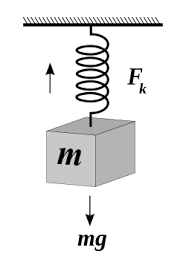
\includegraphics[width=0.75\linewidth]{Images/fuerzas hooke.png}
    \caption{Diagrama de fuerzas inicial}
    \label{Diagrama fuerzas}
\end{wrapfigure}

Cuando el sistema alcanza el equilibrio después de colgar la masa tenemos la siguiente relación:

\begin{equation}
    mg = k\Delta x
    \label{Met estatico}
\end{equation}

Cuando se provoca una nueva deformación el sistema abandona el equilibrio y comienza a oscilar siguiendo un M.A.S. El movimiento ondulatorio se puede modelizar a partir de la ecuación de su posición, que nos permite conocer su velocidad y su aceleración derivando:

\begin{equation}
    \left\{ \begin{array}{l}
        x(t) = A \cos (\varphi - \omega t) \\
        v(t) = \frac{dx}{dt} = -A \omega \sin (\varphi - \omega t) \\
        a(t) = \frac{d^2x}{dt^2} = -A \omega^2 \cos (\varphi - \omega t)
        \end{array}
    \right.
\end{equation}

A partir de estas ecuaciones podemos conocer la aceleración en función de la posición y de la velocidad angular. Si relacionamos por medio de la 2ª ley de Newton la fuerza (Ley de Hooke), con la aceleración obtenemos la siguiente relación:

\begin{equation}
    \begin{gathered}
    a = -\omega^2 x \Rightarrow m\overbrace{(-\omega^2x)}^a = \overbrace{-kx}^F \Rightarrow \omega = \sqrt{\frac{k}{m}} \\
    \omega = \frac{2\pi}{T} \Rightarrow T= 2\pi \sqrt{\frac{m}{k}}
    \end{gathered}
    \label{Met dinamico}
\end{equation}

Donde $T$ representa el período de oscilación del muelle.

\par A partir de estas relaciones podemos calcular la constante elástica del muelle de dos formas diferentes, por el método estático o por el método dinámico. El método estático se basa en la Ec.\ref{Met estatico}, midiendo la deformación que provoca una determinada masa. Por otra parte, el método dinámico se basa en la Ec.\ref{Met dinamico}, midiendo los diferentes períodos de oscilación que provocan diferentes masas. El objetivo de la primera parte de la práctica será determinar la constante elástica $k$ de un muelle a partir de estos dos métodos.

\par En la segunda parte de la práctica abordaremos las aplicaciones de un muelle para la determinación de la densidad de diferentes materiales (Sólidos y líquidos). Partiremos de la posición de equilibrio del muelle con una masa $m$ colgando, como en la Fig.\ref{Diagrama fuerzas}. El fundamento teórico de esta parte será la combinación del principio de Arquímedes con la ley de Hooke. El principio de Arquímedes nos afirma que si sumergimos un cuerpo total o parcialmente en un líquido este sufrirá un empuje hacia arriba igual al peso del fluido desalojado. Por tanto, si sumergimos nuestra masa $m$ en un líquido esta sufrirá un empuje vertical y alcanzará una nueva posición de equilibrio con una deformación menor. Las fuerzas que actúan sobre la masa $m$ en esta nueva situación de equilibrio son:

\begin{equation}
    \sum \vec{F} = 0 \Rightarrow \vec{P} + \vec{F}_k + \vec{E} = 0
\end{equation}

Donde $\vec{P}$ es el peso, $\vec{F}_k$ es la fuerza de recuperación y $\vec{E}$ es el empuje que ejerce el líquido. Si trabajamos con los módulos de las fuerzas y expresamos las masas en función de la densidad ($\rho = \frac{m}{V}$) tenemos que:

\begin{equation}
    \overbrace{\rho_s V_s g}^{\vec{P}} = \overbrace{\rho_L V_s g}^{\vec{E}} + \overbrace{k \Delta x'}^{\vec{F}_k} \Rightarrow \rho_s V_s g - \rho_L V_s g = k\Delta x'
\end{equation}

Si restamos esta ecuación a la Ec.\ref{Met estatico} expresada en función de la densidad ($\rho_s V_s g = k\Delta x$) obtenemos que:

\begin{equation}
    \rho_L V_s g = k (\Delta x -\Delta x')
    \label{Relacion sol liquido}
\end{equation}

Si dividimos la Ec.\ref{Met estatico} en función de la masa entre la Ec.\ref{Relacion sol liquido} obtenemos que:

\begin{equation}
    \rho_s = \rho_L \frac{\Delta x}{\Delta x - \Delta x'}
    \label{Densidad sol}
\end{equation}

Para la determinación de la densidad del líquido solo tendríamos que despejar su valor de la ecuación anterior:

\begin{equation}
    \rho_L = \rho_s \frac{\Delta x- \Delta x'}{\Delta x}
    \label{Densidad liq}
\end{equation}

En la última parte de la práctica trataremos de determinar el valor de la gravedad mediante la caída libre de un objeto.

\begin{figure}[h!]
    \centering
    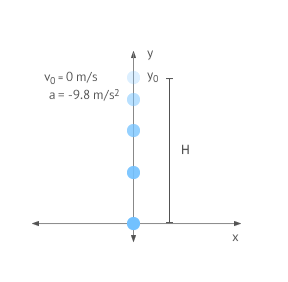
\includegraphics[width=0.5\linewidth]{Images/caidalibre.png}
    \caption{Caída libre ideal de un cuerpo}
\end{figure}

Para ello partiremos de un objeto al que someteremos a una caída libre ideal, despreciando el efecto del rozamiento que ejerce el aire. Un cuerpo en una caída libre ideal sigue un MRUA en el eje $Y$ que se puede modelizar fácilmente con la siguiente ecuación:

\begin{equation}
    y = y_0 +v_0t +\frac{1}{2} at^2 \Rightarrow y = h -\frac{1}{2}gt^2 \overbrace{\Rightarrow}^{y=0} t = \sqrt{\frac{2h}{g}}
    \label{Formula C.L}
\end{equation}

\section{Materiales y metodología}

\subsection{Determinación de la constante elástica de un muelle}

En la primera parte de la práctica determinaremos el valor de la constante elástica de nuestro muelle mediante los dos métodos antes descritos, el método estático y el método dinámico. En el método estático mediremos la relación entre la fuerza que soporta el muelle y su deformación mientras que en el método dinámico mediremos la relación entre la masa que cuelga del muelle y su período. Los materiales empleados para ambas mediciones fueron los siguientes:

\begin{itemize}
    \item Muelle pendurado de un soporte
    \item Pesas de diferentes calibres colgadas de un portapesas
    \item Balanza para medir la masa de las diferentes pesas
    \item Regla vertical para medir la deformación, empleada en el método estático
    \item Cronómetro, empleado para medir el período en el método dinámico
\end{itemize}

\begin{wrapfigure}{r}{0.4\textwidth}
    \centering
    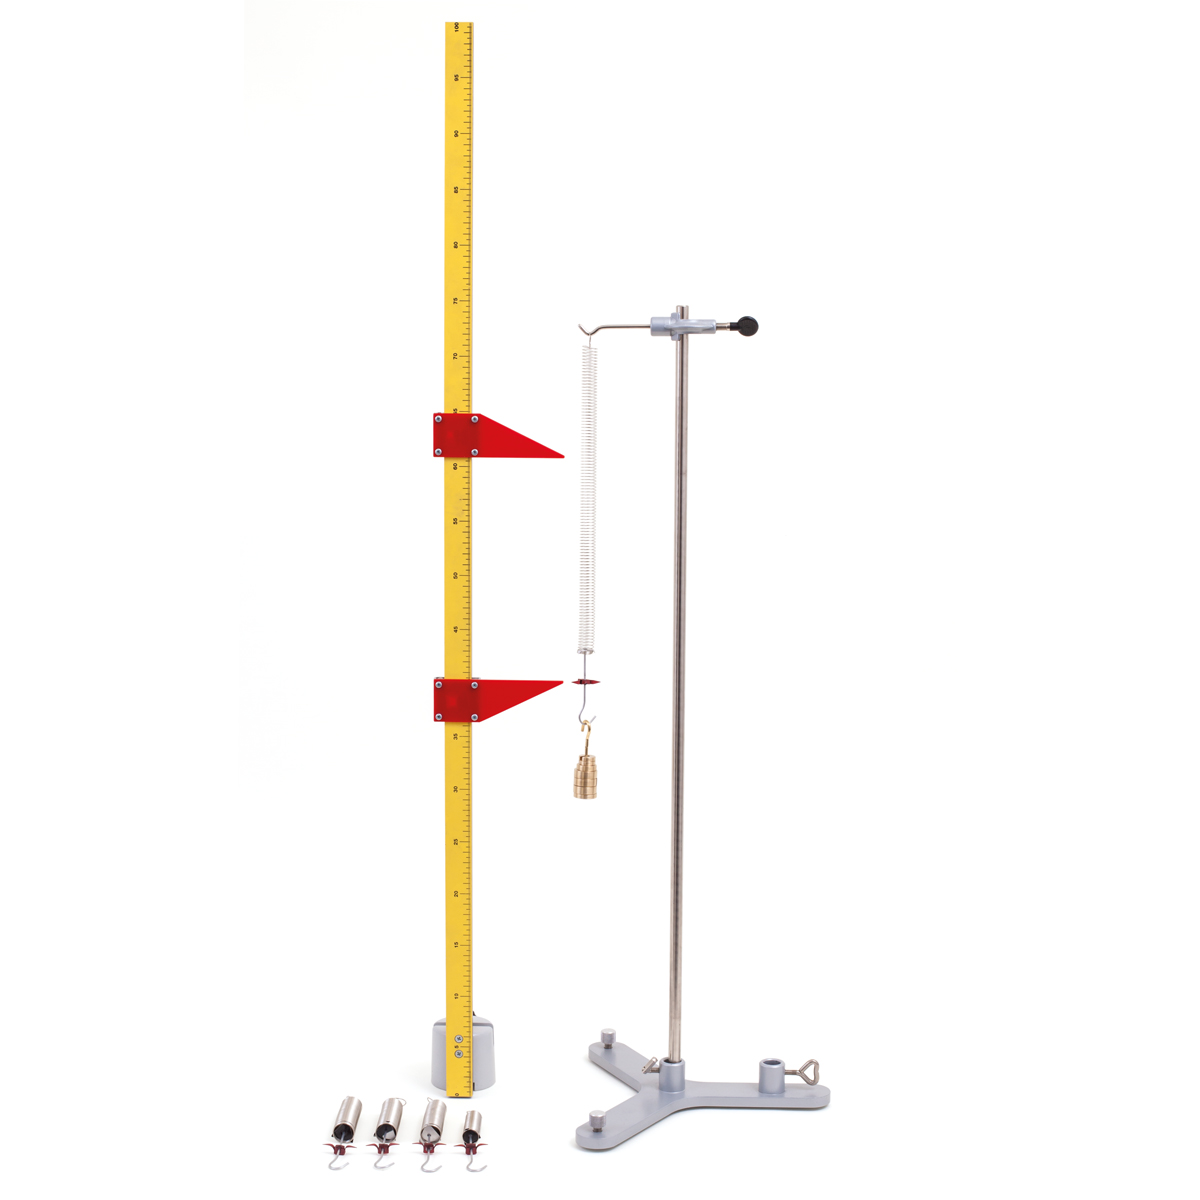
\includegraphics[width=0.95\linewidth]{Images/Ley de hooke.jpg}
    \caption{Montaje experimental para el método estático}
    \label{Montaje estatico}
\end{wrapfigure}

En primer lugar determinamos el valor de la constante elástica por el método estático, adoptando la configuración experimental que se puede ver en la Fig.\ref{Montaje estatico}.
Para determinar la constante decidimos tomar 10 medidas de la deformación que producen diez masas diferentes. Para ello realizaremos una regresión lineal simple sin término independiente por el método de los mínimos cuadrados, representando la fuerza en función de la deformación, ya que siguen una relación lineal como observamos en la Ec.\ref{Met estatico}. La pendiente de la recta ($F=\mathbf{b}\Delta x$) se corresponderá con la constante elástica del muelle. Las incertidumbres con las que trabajaremos en este caso son aquellas que proceden de nuestras medidas directas de las masas y las deformaciones.

\begin{itemize}
    \item La incertidumbre de la masa viene dada por la precisión instrumental de la balanza y será la misma para todas las masas medidas de forma directa durante la práctica. Esta incertidumbre está directamente relacionada con la del peso:
    \begin{equation}
        s(m) = 0,01 \; g = 0,00001 \; kg \Rightarrow s(F) =9,8\cdot s(m) = 0,00098 \; N
        \label{Inc peso}
    \end{equation}
    \item La incertidumbre de la deformación viene dada por la precisión instrumental de la regla, que es de 1 mm. No obstante, en este caso consideramos que la incertidumbre es algo mayor, pues el aparato de medida y el muelle no estaban físicamente pegados y la incertidumbre dependerá de la precisión que tengamos a la hora de tomar las medidas. Es por ello que hemos decidido tomar como incertidumbre de la medida de la regla es de 2 mm. La deformación la mediremos de forma indirecta, fijando un valor de $x_0$ (El punto de equilibrio) como cero y medir lo que se deforma respecto de ese cero restando las medidas según la siguiente ecuación:
    \begin{equation}
        \Delta x = x - x_0
        \label{Deformación}
    \end{equation}

    Por tanto la incertidumbre de la deformación la obtenemos de forma indirecta a partir de la siguiente ecuación:

    \begin{equation}
        s(\Delta x) = \sqrt{\left (\frac{\partial \Delta x}{\partial x}\right )^2s^2(x) + \left (\frac{\partial \Delta x}{\partial x_0}\right )^2s^2(x_0)} = \sqrt{2s^2(x)} = 2\sqrt{2} = 2,8 \; mm
        \label{Inc deformacion}
    \end{equation}
\end{itemize}

El segundo método empleado para determinar la constante elástica fue el método dinámico, que se basa en la relación entre el período de oscilación y la masa que cuelga del muelle, como vimos en la Ec.\ref{Met dinamico}. Si elevamos ambos miembros de esta ecuación al cuadrado obtenemos la siguiente relación:

\begin{equation}
    T^2 = \frac{1}{k} 4 \pi^2 m
\end{equation}

De esta forma podemos ver que existe una clara relación lineal entre las magnitudes $T^2$ y $4\pi^2m$, donde $\frac{1}{k}$ es la pendiente de la propia recta. Para calcular la pendiente de esta recta realizaremos un ajuste simple sin término independiente ($y=bx$) por el método de los mínimos cuadrados de $T^2$ frente a  $4\pi^2m$. La incertidumbre asociada a la masa es la misma, por lo que la incertidumbre asociada a la variable independiente ($4\pi^2m$) es:

\begin{equation}
    s(4\pi^2m) = 4\pi^2s(m) = 0.39 \; g
\end{equation}

La medida del período de oscilación se realizó de forma directa con un cronómetro y para darle mayor fiabilidad a la medida cronometramos un intervalo de tiempo equivalente a diez períodos ($10T$). De esta forma reducimos en un orden de magnitud la incertidumbre de la medida al tener que dividirla entre 10. La incertidumbre de cada medida directa que tomamos ($10T$) será el tiempo de reacción medio de un ser humano, que manda frente a la precisión instrumental del cronómetro. El valor que tomaremos como referencia será el tiempo medio de reacción frente a un estímulo visual que es de $0,25$ s. Por tanto las incertidumbres correspondientes son:

\begin{equation}
    \begin{gathered}
        s(10T) = 0,25 \; s \Rightarrow s(T) = 0,025 \; s \\
        s(T^2) = \sqrt{\left (\frac{\partial T^2}{\partial T} \right )^2s^2(T)} = 2T\cdot s(T) = 0,05 \cdot T \; s
        \label{Inc T^2} 
    \end{gathered}
\end{equation}

A partir del ajuste podremos calcular el valor de la constante elástica del muelle y compararemos los resultados obtenidos por ambos métodos.

\subsection{Determinación de densidades de diferentes materiales}

En este apartado de la práctica trataremos de determinar la densidad de varios sólidos y un líquido. Para ello empleamos los siguientes materiales:

\begin{itemize}
    \item Muelle pendurado de un soporte
    \item Pesas de densidad desconocida y una balanza
    \item Un líquido de densidad conocida, agua, y otro de densidad desconocida, alcohol.
    \item Regla vertical para medir la deformación
\end{itemize}



\begin{wrapfigure}{l}{0.4\textwidth}
    \centering
    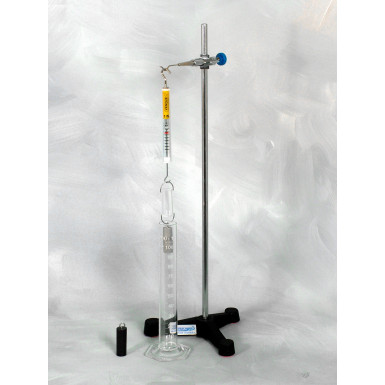
\includegraphics[width=0.95\linewidth]{Images/hooke+arquimedes.jpg}
    \caption{Montaje experimental para la determinación de densidades}
    \label{Hooke+arquimedes}
\end{wrapfigure}

Como explicamos en la introducción, nos vamos a valer del principio de Arquímedes para determinar diferentes densidades. El objetivo fundamental será cuantificar el efecto del empuje del líquido en la deformación, que será menor que en ausencia de líquido. Para ello mediremos la deformación que sufre el muelle cuando de él cuelga una masa $m$, $\Delta x$, y la deformación cuando esa misma masa $m$ está sumergida en un líquido de densidad conocida, $\Delta x'$. El montaje experimental empleado puede verse en la siguiente Fig.\ref{Hooke+arquimedes}. De esta forma podremos calcular la densidad del material del que está hecho esa misma masa $m$, aplicando la Ec.\ref{Densidad sol}. Para calcular la densidad de un líquido debemos realizar las mismas medidas con un sólido de densidad conocida (Usaremos la calculada anteriormente) y aplicaremos la Ec. \ref{Densidad liq}. La incertidumbre asociada a las deformaciones es la misma con la que trabajamos en el apartado anterior, reflejada en la Ec.\ref{Inc deformacion}. Por otro lado, tomaremos la densidad conocida como una constante y calcularemos la densidad del material desconocido a partir de propagación de incertidumbres:

\begin{itemize}
    \item Aplicando propagación de incertidumbres a la Ec.\ref{Densidad sol} obtenemos la incertidumbre de la densidad del sólido:
    \begin{equation}
        s(\rho_s)=\sqrt{\left (\frac{-\rho_L \Delta x'}{(\Delta x -\Delta x')^2} \right )^2s^2(\Delta x) + \left (\frac{\rho_L \Delta x}{(\Delta x - \Delta x')^2}\right )^2s^2(\Delta x')}
        \label{Inc densidad solido}
    \end{equation}
    \item Aplicando propagación de incertidumbres a la Ec.\ref{Densidad liq} obtenemos la incertidumbre de la densidad del líquido:
    \begin{equation}
        s(\rho_L) = \sqrt{ \left (\frac{\rho_s\Delta x'}{(\Delta x)^2}\right )^2s^2(\Delta x) + \left (\frac{-\rho_s}{\Delta x} \right )^2s^2(\Delta x') + \left (\frac{\Delta x -\Delta x'}{\Delta x}\right )^2s^2(\rho_s)}
        \label{Inc densidad liquido}
    \end{equation}
\end{itemize}

\subsection{Determinación del valor de la gravedad}

El último apartado de la práctica consiste en determinar el valor de la gravedad a partir de una caída libre controlada que suponemos ideal. El material empleado fue el siguiente:

\begin{itemize}
    \item Bola metálica
    \item Aparato dotado de un electroimán y un sensor de movimiento
    \item Regla milimetrada
\end{itemize}

\begin{wrapfigure}{r}{0.4\textwidth}
    \centering
    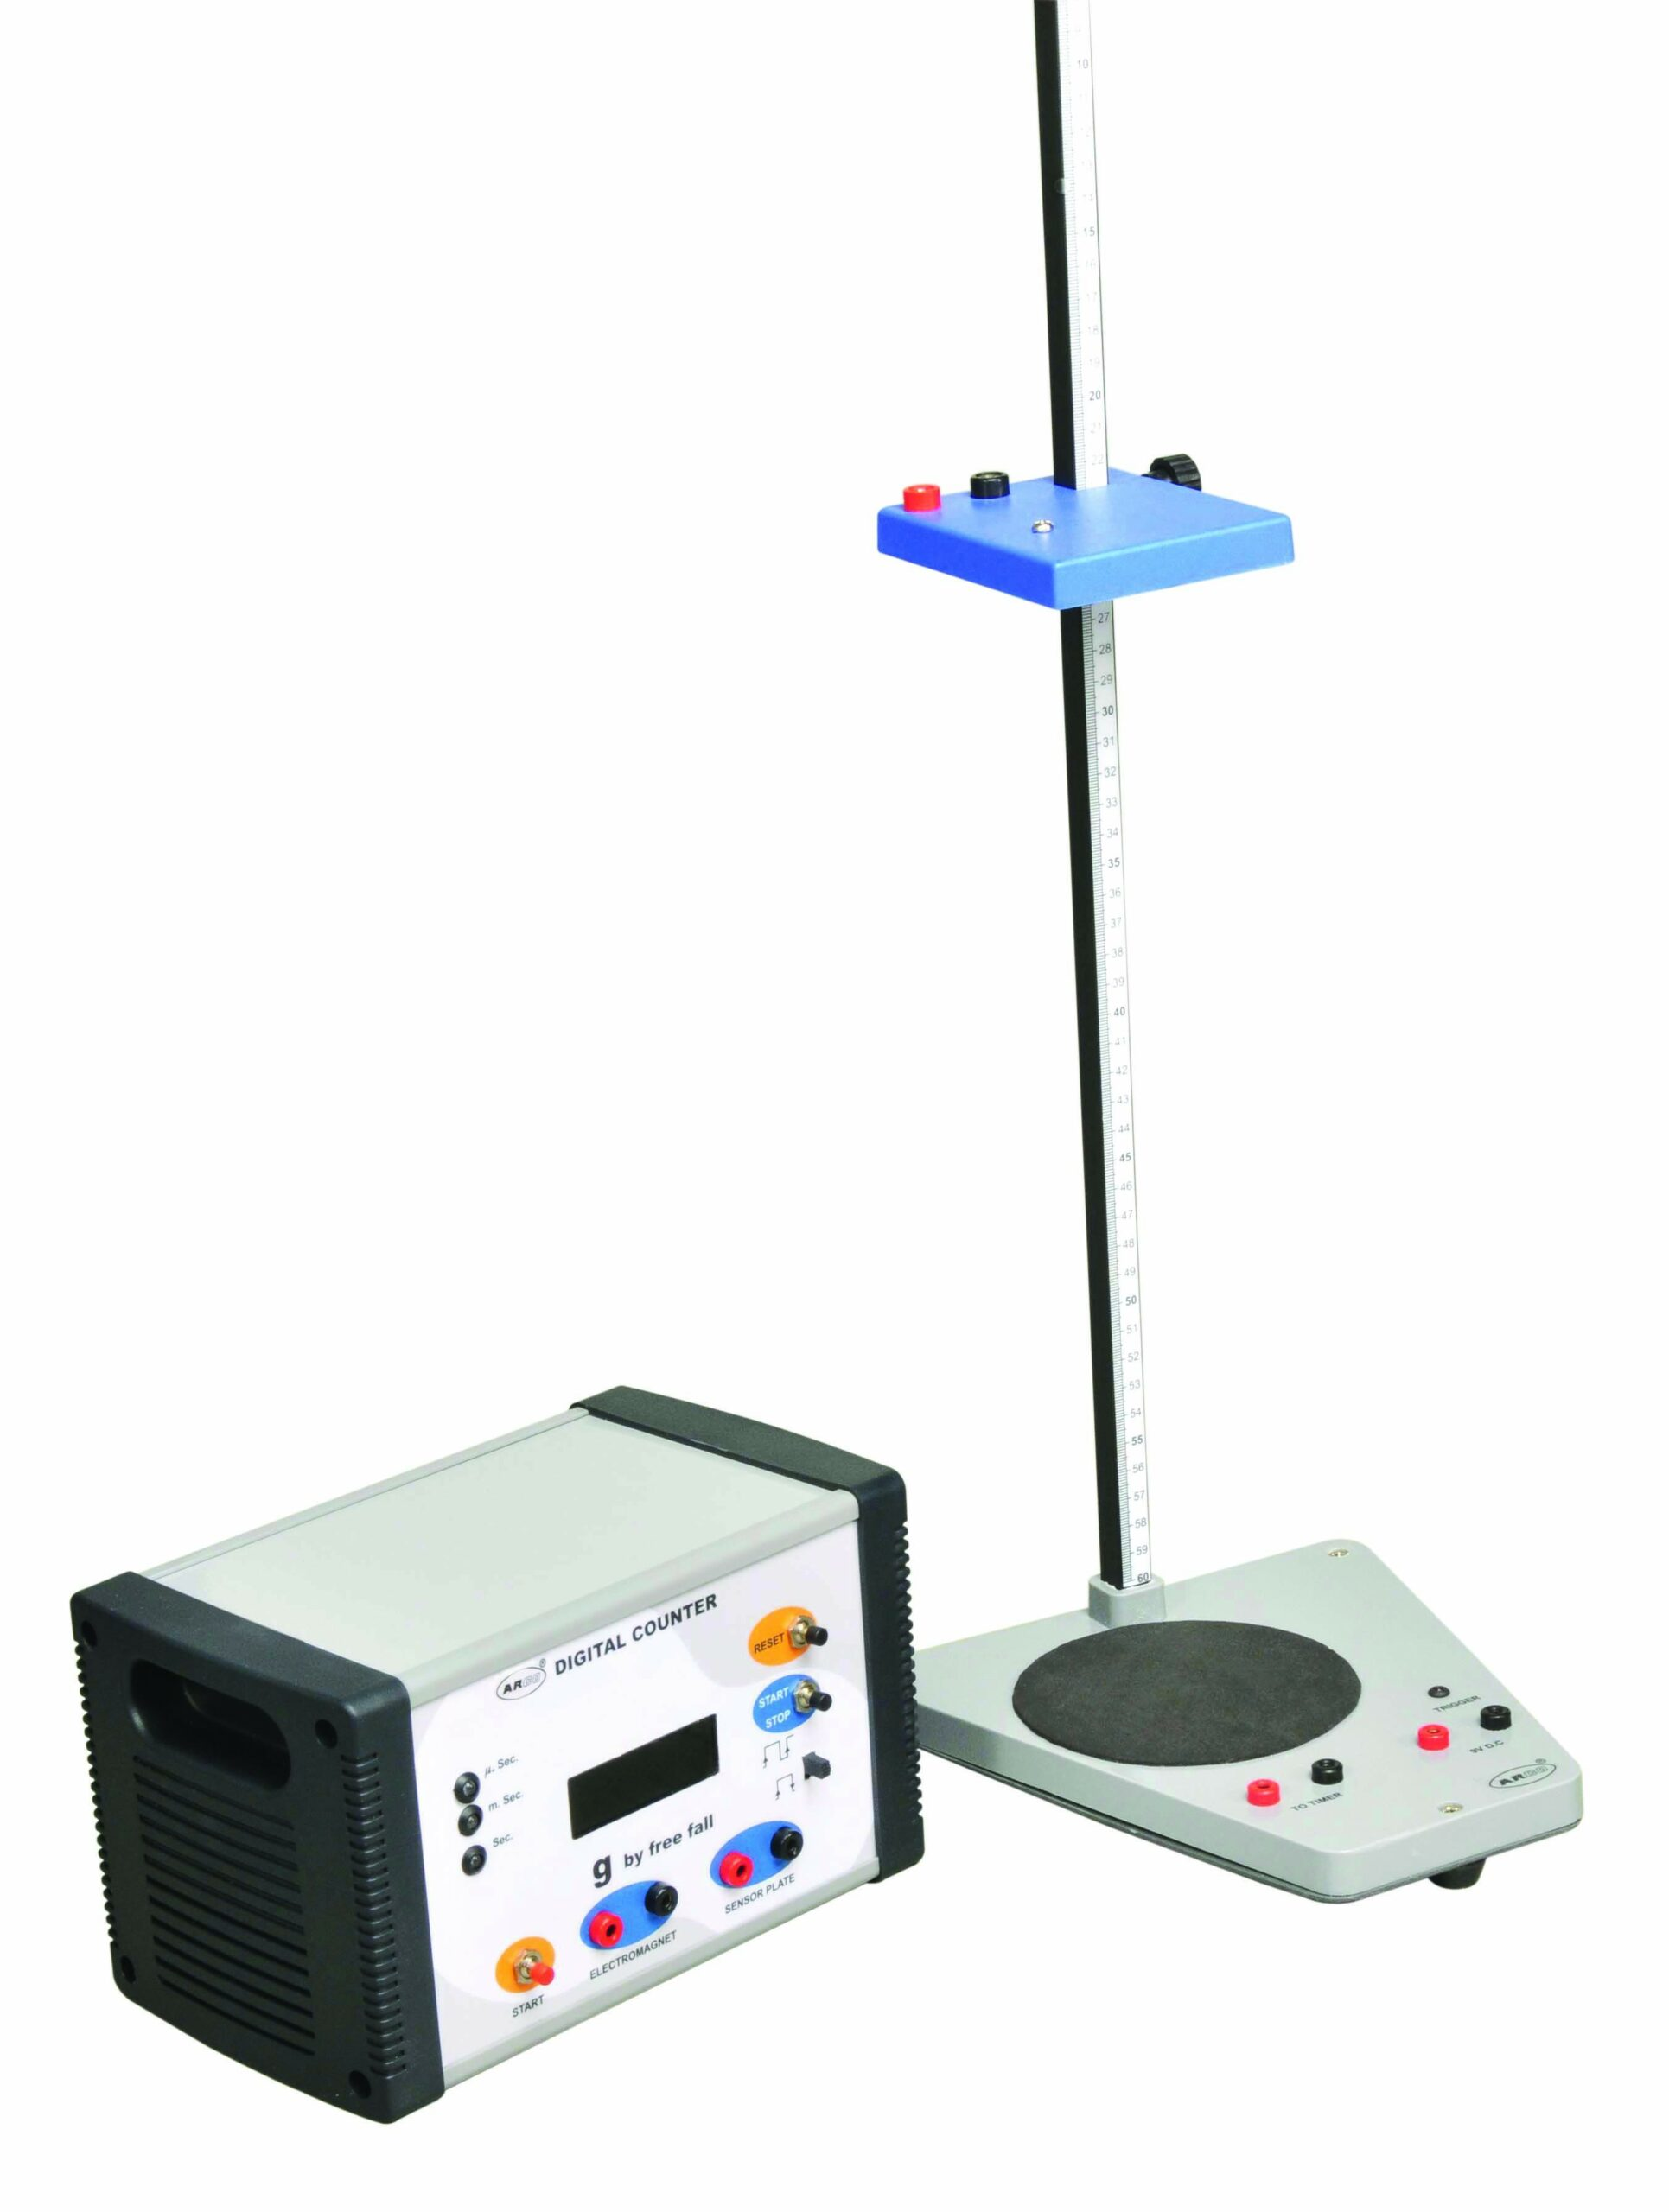
\includegraphics[width=0.7\linewidth]{Images/caidalibreaparato.jpg}
    \caption{Aparato para medir el tiempo de caída}
    \label{Montaje caida}
\end{wrapfigure}

El procedimiento llevado a cabo es muy sencillo, pues contábamos con un aparato de medida (Fig.\ref{Montaje caida}) dotado de un electroimán que soportaba la bola hasta que llegaba la señal para que se soltara y comenzaba nuestra caída libre. En ese preciso instante en que comenzaba la caída se activaba el contador del tiempo de caída gracias al sensor de movimiento, que paraba el contador cuando la bola llegaba a la base del aparato. Para calcular el valor de $g$ tomamos 10 medidas del tiempo de caída para diferentes alturas y realizamos una regresión lineal simple sin término independiente:

\begin{equation}
    t = \sqrt{\frac{2h}{g}} \Rightarrow 2h = gt^2
    \label{Ajuste gravedad}
\end{equation}

A partir de esta expresión ya tenemos nuestra relación lineal (Entre $2h$ y $t^2$) con la que podremos realizar nuestro ajuste por mínimos cuadrados a una recta del tipo $2h=bt^2$ donde la pendiente de la recta se corresponde con el valor de la gravedad. Las incertidumbres que debemos tener en cuenta son las siguientes:

\begin{itemize}
    \item La incertidumbre de la altura viene dada por la precisión instrumental de la regla:
    \begin{equation}
        s(h) = 0,001\; m \Rightarrow s(2h) = 0,002 \; m
    \end{equation}
    \item La incertidumbre del tiempo de caída viene dada por la incertidumbre del sensor, este valor nos ayudará a calcular la incertidumbre de $t^2$ a partir de propagación de incertidumbres:
    \begin{equation}
        s(t) = 0.00001 \; s \Rightarrow s(t^2)= 2t \cdot s(t) = 0.00002 \cdot t \; s
        \label{Inc Tcuadrado}
    \end{equation}
\end{itemize}

\newpage

\section{Análisis de datos}

\subsection{Determinación de la constante elástica del muelle}

\subsubsection{Método estático}

Como hemos mencionado anteriormente, para el método estático hemos tomado diez medidas de la deformación que producen diferentes masas. En la siguiente tabla podemos ver esos datos, así como la fuerza producida por esa masa:

\begin{table}[h!]
    \centering
    \begin{tabular}{|c|c|c|}
    \hline
    Masa (g) & F (N) ($F=mg$) & $\Delta x$ (m) \\ \hline
    10,2   & 0,09996 & 0,033 \\ \hline
    30,25  & 0,29645 & 0,099 \\ \hline
    50,27  & 0,49265 & 0,163 \\ \hline
    70,24  & 0,68835 & 0,227 \\ \hline
    80,2   & 0,78596 & 0,26  \\ \hline
    90,22  & 0,88416 & 0,291 \\ \hline
    100,01 & 0,98010 & 0,322 \\ \hline
    105,04 & 1,02939 & 0,34  \\ \hline
    110,07 & 1,07869 & 0,355 \\ \hline
    115,15 & 1,12847 & 0,372 \\ \hline
    \end{tabular}
    \caption{Datos experimentales medidos en el método estático}
    \label{Datos estatico}
\end{table}

A partir de la regresión lineal de $F$ frente a $\Delta x$ obtuvimos las siguientes magnitudes:

\begin{equation}
    \begin{gathered}
        b =  3.0335 \; N \cdot m^{-1} \\
        s(b) = 0.0026 \; N \cdot m^{-1} \\
        r =  0.999996 \\
        s =  0.0023
    \end{gathered}
\end{equation}

En la siguiente gráfica podemos ver respresentados los datos experimentales y la recta de regresión:

\newpage

\begin{figure}[h!]
    \centering
    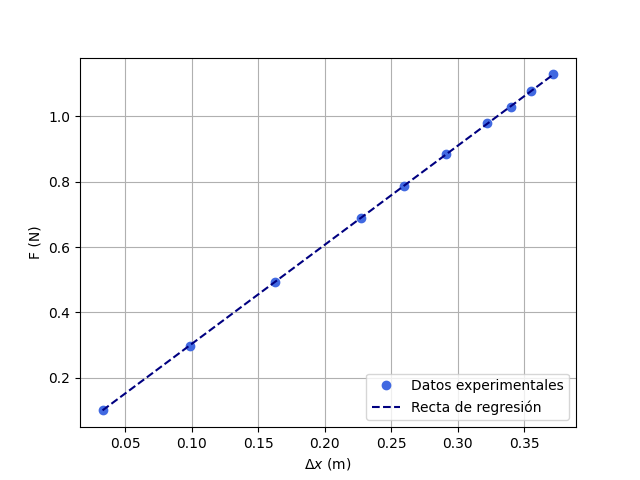
\includegraphics[width=0.75\linewidth]{Images/RegEstatico.png}
    \caption{Datos experimentales y recta de regresión del método estático}
\end{figure}

Finalmente, el valor de la constante elástica del muelle se corresponde con la pendiente de la recta, como demostramos antes, por lo que su valor es:

\begin{equation}
    k = 3.0335 \pm 0.0026 \; N \cdot m^{-1}
\end{equation}

\subsubsection{Método dinámico}

Para el método dinámico hemos tomado diez medidas del período de oscilación (En concreto de $10T$) para cada una de las masas empleadas anteriormente. Los datos recogidos figuran en la siguiente tabla acompañados de su respectiva incertidumbre, en el caso de $T^2$:

\newpage

\begin{table}[h!]
    \centering
    \begin{tabular}{|c|c|c|c|c|}
    \hline
    Masa (g) & $10T \; (s)$ & $T \; (s)$ & $T^2 \; (s^2) $&   $s(T^2) \; (s^2)$\\ \hline
    10,20   & 4,24  & 0,424 & 0,180 & 0,021 \\ \hline
    30,25  & 7,07  & 0,707 & 0,500 & 0,035 \\ \hline
    50,27  & 8,47  & 0,847 & 0,717 & 0,042 \\ \hline
    70,24  & 9,97  & 0,997 & 0,994 & 0,050  \\ \hline
    80,20   & 10,56 & 1,056 & 1,115 & 0,053 \\ \hline
    90,22  & 11,22 & 1,122 & 1,259 & 0,056 \\ \hline
    100,01 & 11,72 & 1,172 & 1,374 & 0,059 \\ \hline
    105,04 & 12,07 & 1,207 & 1,457 & 0,060  \\ \hline
    110,07 & 12,19 & 1,219 & 1,486 & 0,061 \\ \hline
    115,15 & 12,62 & 1,262 & 1,593 & 0,063 \\ \hline
    \end{tabular}
    \caption{Datos experimentales obtenidos a partir del método dinámico}
    \label{Datos dinamico}
\end{table}

A partir de estos datos vamos a realizar nuestra regresión lineal de $T^2$ frente a $4\pi^2m$, como se ha mencionado anteriormente. Como los valores de $T^2$ presentan incertidumbres variables cabría la posibilidad de realizar un ajuste ponderado. No obstante, como la variación de las incertidumbres es pequeña, no llega siquiera a un orden de magnitud, vamos a realizar un ajuste simple, que nos proporcionará una aproximación muy buena del resultado. Los parámetros obtenidos fueron los siguientes:

\begin{equation}
    \begin{gathered}
        b = 0.3512 \; m\cdot N^{-1}\\
        s(b) = 0.0033 \; m\cdot N^{-1}\\
        r =  0.9996 \\
        s =  0.034
    \end{gathered}
\end{equation}

Como mencionamos anteriormente, la pendiente de esta recta es $\frac{1}{k}$, por lo que la constante elástica y su incertidumbre tienen la siguiente expresión:

\begin{equation}
    \begin{gathered}
        k = \frac{1}{b} = 2.847 \; N\cdot m^{-1} \\
        s(k) = \sqrt{\left (\frac{\partial k}{\partial b} \right )^2s^2(b)} = \frac{s(b)}{b^2} = 0.027 \; N\cdot m^{-1}
    \end{gathered}
\end{equation}

En la siguiente gráfica podemos ver una representación de los datos experimentales y de nuestra recta de regresión:

\begin{figure}[h!]
    \centering
    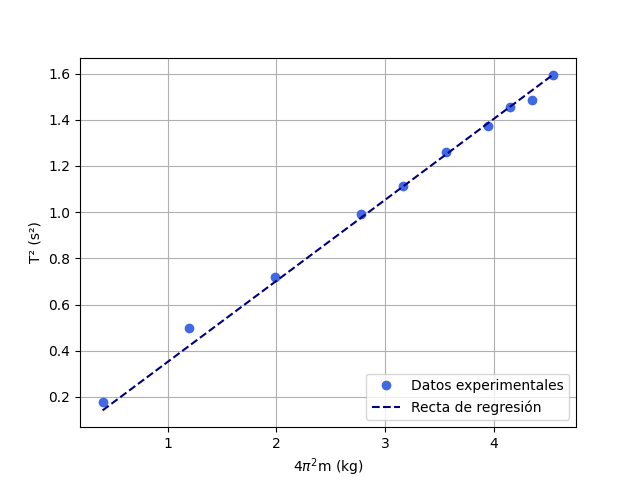
\includegraphics[width=0.75\linewidth]{Images/RegDinamico.png}
    \caption{Datos experimentales y recta de regresión del método dinámico}
\end{figure}

Finalmente, podemos ver que el valor de nuestra constante difiere un poco al calculado por el método estático. Esta pequeña diferencia podría explicarse por el hecho de haber realizado una regresión lineal simple en vez de ponderada, que era lo que el problema pedía inicialmente al estar tratando con incertidumbres variables. Otra posible explicación de esta diferencia es un cierto error en la medida, pues muchas veces las oscilaciones no eran perfectas, si no que presentaban mucha irregularidad.



\subsection{Determinación de densidades}

\subsubsection{Sólidos}

Para la determinación de la densidad de sólidos contábamos con tres pesas de densidad desconocida, $m_1$, $m_2$ y $m_3$, y un líquido de densidad conocida, el agua $(\rho = 1000 \; kg\cdot m^{-3}=1 \; g\cdot mL^{-1})$. En la siguiente tabla podremos ver los valores de la deformación medidos ($\Delta x$), así como las deformaciones con los sólidos sumergidos en agua ($\Delta x'$), y la densidad y su incertidumbre (Calculadas a partir de la Ec.\ref{Densidad sol} y de la Ec.\ref{Inc densidad solido}):

\begin{table}[h!]
    \centering
    \begin{tabular}{c|c|c|c|c|}
    \cline{2-5}
    \multicolumn{1}{l|}{}        & $\Delta x \; (m)$ & $\Delta x' \; (m)$ & $\rho_s \; (g\cdot cm^{-3})$ & $s(\rho_s) \; (g\cdot cm^{-3})$ \\ \hline
    \multicolumn{1}{|c|}{Masa 1} & 0,16  & 0,102 & 8,40 & 0,59 \\ \hline
    \multicolumn{1}{|c|}{Masa 2} & 0,445 & 0,392 & 2,76 & 0,16 \\ \hline
    \multicolumn{1}{|c|}{Masa 3} & 0,476 & 0,425 & 9,33 & 0,69 \\ \hline
    \end{tabular}
    \caption{Datos experimentales y cálculo de la densidad}
    \label{Datos dens sol}
\end{table}

Para el contraste de resultados nos podemos fijar solo en un valor, el de la masa 2, que era la única hecha de un material conocido, aluminio. La densidad real del aluminio es de $2,7 \; g\cdot cm^{-3}$, que está muy próximo al valor calculado experimentalmente y entra dentro de su rango de incertidumbre.

\subsubsection{Líquidos}

En este apartado tratamos de determinar la densidad, \textit{a priori} desconocida, de un líquido, el alcohol. Para ello tomamos las mismas medidas que en el apartado anterior, pero sumergiendo las tres mismas masas en alcohol en vez de en agua. De esta forma mediremos las diferentes deformaciones que se producen con las pesas al aire o sumergidas. Aplicando la Ec.\ref{Densidad liq} y la Ec.\ref{Inc densidad liquido} podemos calcular la densidad del alcohol con su incertidumbre asociada:

\subsection{Determinaación de la gravedad}

El último apartado de la práctica consistía en determinar el valor de la aceleración gravitatoria $g$ a partir de la caída libre ideal. Tomamos diez valores de referencia de tiempo de caída y altura, que representaremos en la siguiente tabla.Las incertidumbres de $t^2$ vienen dada spor la Ec.\ref{Inc Tcuadrado}:

\begin{table}[h!]
    \centering
    \begin{tabular}{|c|c|c|c|c|}
    \hline
    $h \; (m)$ & $2h \; (m)$ & $t \; (s)$ & $t^2 \; (s^2)$ & $s(t^2) \; (s^2)$ \\ \hline
    0,380 & 0,760 & 0,27488 & 0,0755590 & 0,0000055 \\ \hline
    0,400  & 0,800  & 0,28261 & 0,0798684 & 0,0000057 \\ \hline
    0,420 & 0,840 & 0,29176 & 0,0851239 & 0,0000058 \\ \hline
    0,460 & 0,920 & 0,29593 & 0,0875746 & 0,0000059 \\ \hline
    0,480 & 0,960 & 0,30416 & 0,0925133 & 0,0000061 \\ \hline
    0,500  & 1,000    & 0,31177 & 0,0972005 & 0,0000062 \\ \hline
    0,520 & 1,040 & 0,31880  & 0,1016334  & 0,0000064 \\ \hline
    0,540 & 1,080 & 0,32952 & 0,1085834  & 0,0000066 \\ \hline
    0,560 & 1,120 & 0,33338 & 0,1111422 & 0,0000067 \\ \hline
    0,580 & 1,160 & 0,34094 & 0,1162401 & 0,0000068 \\ \hline
    \end{tabular}
    \caption{Datos experimentales de la caída libre}
    \label{Datos gravedad}
\end{table}

A partir de estos datos vamos a realizar una regresión lineal por el método de los mínimos cuadrados de $2h$ frente a $t^2$ para conocer que el valor de $g$, que coincide con la pendiente de la recta. Como en la regresión realizada en el cálculo de $k$ por el método dinámico, cabría la posibilidad de realizar una regresión lineal ponderada. No obstante, la variación de las incertidumbres de $t^2$ es extremadamente pequeña, no llega siquiera al orden de magnitud, por lo que realizaremos una pequeña aproximación empleando una regresión simple sin término independiente. Las magnitudes obtenidas a partir del ajuste fueron las siguientes:

\begin{equation}
    \begin{gathered}
        b =  10.126 \; m \cdot s^{-2} \\
        s(b) = 0.063 \; m \cdot s^{-2} \\
        r =  0.9998 \\
        s =  0.019
    \end{gathered}
\end{equation}

En la siguiente figura podemos ver una representación gráfica de los datos experimentales, así como la recta de regresión:

\begin{figure}[h!]
    \centering
    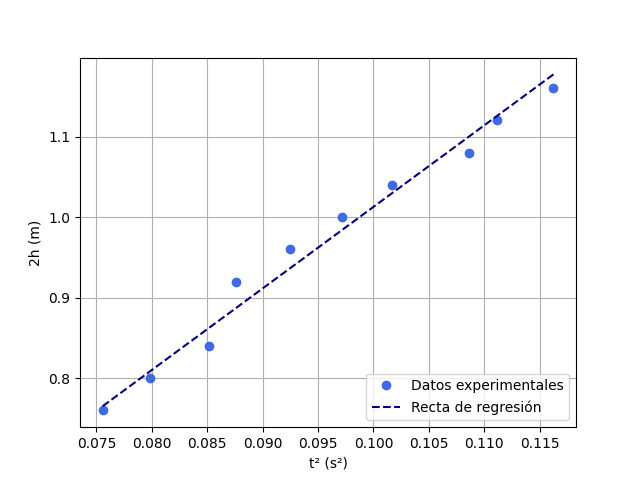
\includegraphics[width=0.75\linewidth]{Images/RegGravedad.png}
    \caption{Datos experimentales y regresión lineal de la caída libre}
\end{figure}

Por tanto el valor final de la aceleración de la gravedad es:

\begin{equation}
    g = 10.126 \pm 0.063 \; m \cdot s^{-2}
\end{equation}

Este valor dista un poco del valor real de $9,807 \; m \cdot s^{-2}$, pero está dentro de un margen razonable para considerar al experimento como verídico.

\section{Conclusiones}

\end{document}